\documentclass[10pt, titlepage]{report}

\usepackage[utf8]{inputenc}
\usepackage[T1]{fontenc}
\usepackage[francais]{babel}

%Caractères spéciaux

\usepackage{lmodern}
\usepackage{amsmath}
\usepackage{amssymb}
\usepackage{mathrsfs}

\usepackage{eurosym} %insertion signe euro
\usepackage{graphicx} %insertion d'images
\usepackage{fancyhdr} %en-tete et pied de page

\title{\bsc{Rapport de la deuxième soutenance}\\Projet flight arena}
\author{mr cube :\\
Vincent \bsc{Rospini-Clerici},\\
Guillaume \bsc{Rebut}\\
%Nikolas \bsc{Miletic}\\
chef de projet : Arthur \bsc{Remaud}}
\date{7 mai 2015}

\pagestyle{fancy}
\fancyhead{}
\fancyfoot{}
\lhead{Rapport de la deuxième soutenance}
\rhead{Projet flight arena}
\lfoot{mr cube}

\begin{document}

\maketitle
\renewcommand{\contentsname}{Sommaire}
\renewcommand{\chaptername}{Partie}

\tableofcontents

\chapter{Rappel de la première soutenance}

A la première soutenance, nous avions présenté une première carte de jeu de base avec un vaisseau déjà fini. Il y avait les déplacements et les tirs du joueur intégrés aux contrôles. Nous avions donc déjà les bases du gameplay, et la physique était bien avancée.\\

Le menu contenait déjà les principaux onglets : jouer, multijoueur, options, quitter. Cependant, certains n'aboutissaient sur rien car le contenu n'avait pas été fait (le multijoueur surtout), mais le menu option avait été entamé avec la gestion du volume qui était conservé en mémoire même après avoir fermé le jeu.\\

Il nous avait été signalé que les déplacements seraient mieux si nous utilisions des quaternions, pour avoir un rendu plus réaliste.\\

\chapter{Retard/Avance par rapport au cahier des charges}

\section{Prévisions}
A l'issue de la première soutenance nous avions prévu pour la seconde soutenance d'améliorer le contenu du jeu en ajoutant de nouvelles modélisations et des paramètres dynamiques, de créer une intelligence artificielle qui fonctionne correctement, et un site web quasiment opérationnel. Le multijoueur en écran scindé, en LAN, ou en réseau devait aussi être ébauché. Le menu des options devait être complété, et il fallait rajouter la sélection du vaisseau au démarrage de la partie.

Le site internet devait être commencé et contenir les informations de base autour du projet.\\

\section{Retard}

\subsection{Intelligence artificielle}
En voulant d'ores et déjà nous concentrer sur le multijoueur, nous avons reporté la finalisation de l'intelligence artificielle à plus tard. L'intelligence artificielle qui est actuellement sur le jeu fonctionne en essayant d'éviter les obstacles mais ne cherche pas à détruire le vaisseau adverse.\\

\subsection{Option changer de touches de commande}

Nous voulions rajouter dans le menu des options la possibilité de choisir ses propres touches sur le clavier pour piloter le vaisseau et faire en sorte que le jeu le retienne. Cependant, nous ignorons totalement comment le faire et aucun site internet ne parle de cela.

Comme Unity, de base, permet au démarrage d'assigner ses touches, et que cela n'est qu'un bonus pas nécessaire, nous avons donc abandonné notre idée de base.\\

\section{Avance}

\subsection{Multijoueur}
Le multijoueur était dans les prévisions la priorité entre la seconde soutenance et la soutenance finale. Mais, nous nous sommes finalement ravisé d'attendre pour le commencer, car notre projet, venant tout d'abord de l'idée de créer un jeu en arène pour que les joueurs puissent s'affronter entre eux. Or, la création d'intelligence artificielle en amont aurait considérablement ralenti l'arrivée d'un multijoueur jouable. Désormais, le jeu est jouable, que ce soit en écran scindé, en LAN.\\

Finalement, l'avance prise sur le multijoueur compense le retard pris dans l'intelligence artificielle : nous avons juste inversé les prévisions entre la deuxième et la dernière soutenance.

\chapter{Travail par membre}
Nous allons vous décrire ce que chaque membre de l'équipe mr cube a fait pendant cette deuxième période, avec leurs difficultés rencontrées et les techniques utilisées.

\section{Guillaume Rebut}

\subsection{Ce que Guillaume doit faire pour la soutenance finale}

\section{Vincent Rospini-Clerici}

\subsection{Création de nouveaux vaisseaux}
Dans le soucis d'ajouter du contenu, deux nouveaux vaisseaux ont été créés sur Blender et textures sur Photoshop. Il s'agit tout d'abord d'un vaisseau qui ferait penser à un jet militaire tout droit venu du futur. L'autre est inspiré du P40, un avion militaire américain utilisé durant la seconde guerre mondiale et auquel Vincent a rajouté des nacelles de missiles et des réacteurs pour lui donner un air à la fois futuriste et ancien. Deux textures ont été crées pour ce dernier vaisseau mais nous nous servirons pour le moment d'une seule d'entre elle pour la première soutenance.\\

\begin{center}
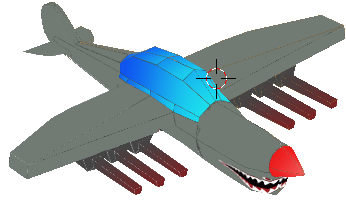
\includegraphics[height=3cm, width=5cm]{sharknado.png}
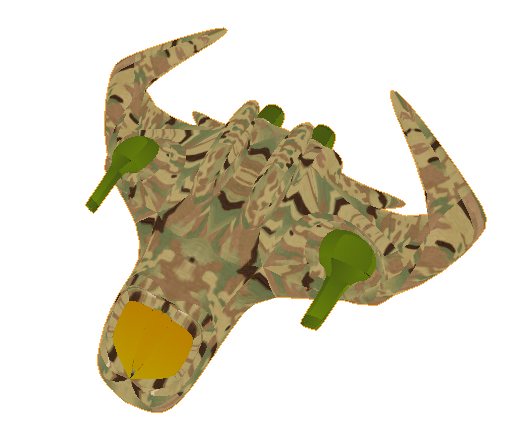
\includegraphics[height=3.5cm, width=5.5cm]{vaisseaumilitaire.png}
\end{center}


\subsection{Ajout des particules des vaisseaux}
Les flammes sortant des réacteurs des vaisseaux ont été rajoutes par le biais de la création de particules qu'offre Unity. Tout d'abord, Vincent a rajouté des éléments de particules pour créer juste des flammes sortant des réacteurs, mais le groupe s'est mis d'accord pour que les réacteurs laissent une trainée après le passage du vaisseau. Cependant, les particules étant contenu dans le \textit{gameobject} du vaisseau, les flammes tournaient lorsque le vaisseau tournait, au lieu de simplement suivre sa trajectoire. Nous avons après quelques recherches sur internet nous avons trouve le paramètre permettant de le faire. Il s'agissait de définir l'espace de simulation au niveau monde et non au niveau de l'objet.\\

\begin{center}
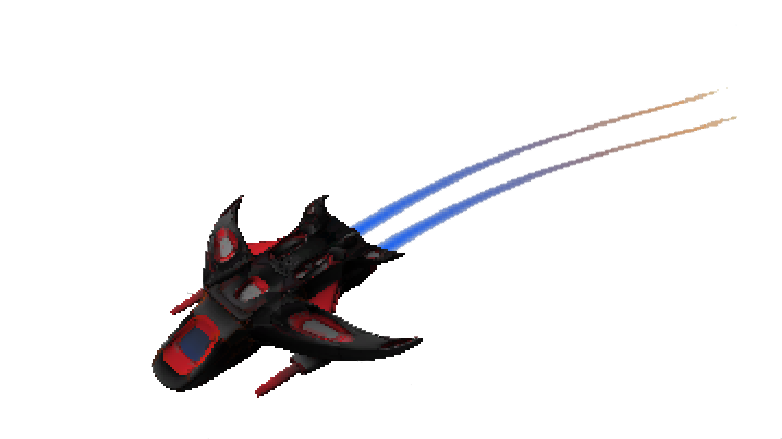
\includegraphics[height=3cm, width=5cm]{vaisseau_bouge.png}
\end{center}

Les trainées laissées par le réacteur sont différentes selon le vaisseau. Par exemple, l'avion laisse une trainée noire de fumée tandis que le vaisseau rouge et noir laisse une trainée bleu rectiligne.De cette façon, les vaisseaux adverses sont plus faciles à reconnaitre parmi les différents éléments de la carte. \\

\subsection{Création du site internet}
Vincent s'est occupé de la création du site internet en vue de la seconde soutenance. Il a décidé de créer le site en langage \textit{HTML} par le biais des logiciels d'adobe, Photoshop et DreamWeaver. Ce dernier est un logiciel permettant d'à la fois modifier directement le code du site et de s'occuper de son coté graphique plus aisément.\\

Il a voulu créer un site avec un design sombre qui rappellerait un ciel étoilé avec de nombreuses images des vaisseaux crées afin de le rendre attirant. Les pages du site ont été désignées sur Photoshop avec des images crées spécialement pour le fond d'écran et pour embellir les pages du site. Le site est prévu pour avoir toutes ses pages traduites en anglais et en français en cliquant simplement sur le drapeau correspondant a la langue voulue. Le site contiendra une page d'accueil,une page pour présenter le jeu, une pour présenter l'équipe et une pour que les visiteurs puissent avoir accès au cahier des charges, à l'exécutable du jeu, et peut-être à d'autres contenus à venir.\\

\begin{center}
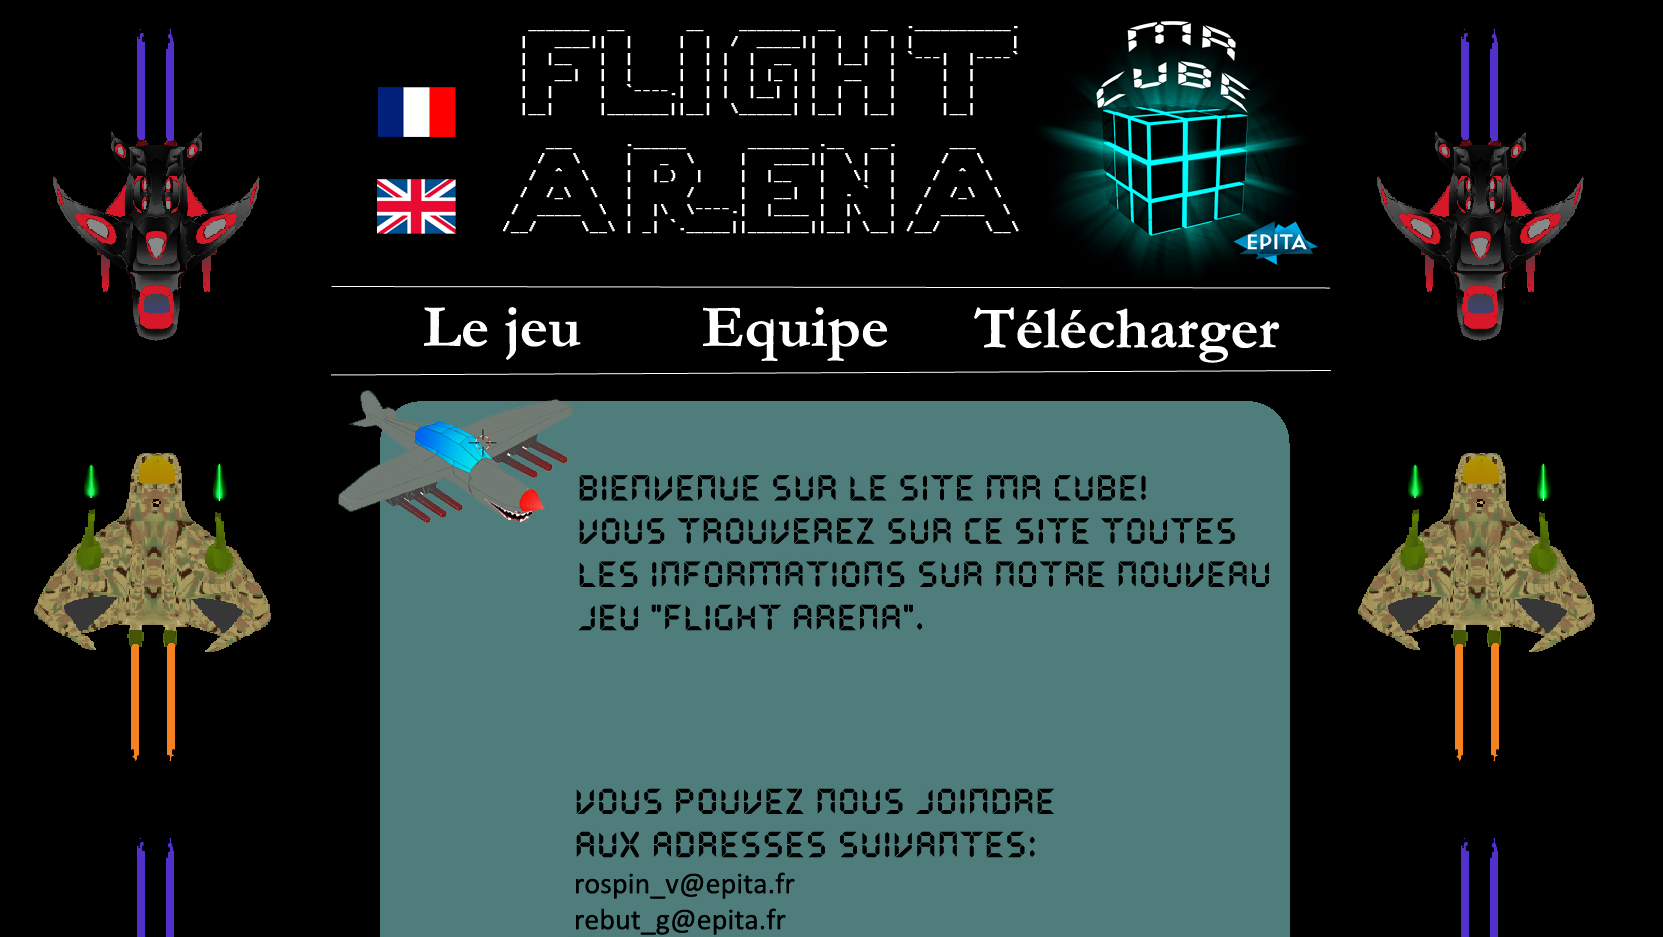
\includegraphics[height=5cm, width=8cm]{site.png}\\
aperçu du site internet
\end{center}

\subsection{Création d'une musique originale}
Nous avons finalement eu le temps et la patience de créer une \textit{original soundtrack} pour le jeu. Vincent a contacté un ami à lui qui fait des études musicales afin de savoir s'il était possible de créer des musiques en coopération avec lui. La réponse étant positive, deux musiques ont été créés à ce jour par notre ami assisté par Vincent par le biais du logiciel Logic Pro. "There's something beyond", une de ces deux musiques a été ajoutée sur Unity et est écoutable dès lors qu'un joueur entre dans la partie. L'autre musique "Vincighilan" sera probablement ajoutée avec l'apparition d'une nouvelle carte ou d'un tutoriel.

\subsection{Ce que Vincent doit faire pour la soutenance finale}
Pour la soutenance finale, le site sera terminé et mis en ligne sur un serveur. La présentation du jeu sera ajoutée sur une nouvelle page du site pour les gens qui le découvrent. Cela permettra aux fans du jeu de se tenir au courant des dernières mises à jour. Des nouveaux éléments de décor seront également créés pour la prochaine carte prévue pour le jeu.\\

La destruction du vaisseau devra être rajoutée dans Unity. Elle est une part très importante du jeu. En sachant que nous n'arrivons pas à implanter la destruction du vaisseau de Blender dans Unity, nous allons donc faire disparaitre le vaisseau quand celui-ci sera détruit et rajouter des particules d'explosion et de debris pour masquer cette disparition soudaine. De ce fait, cette destruction sera réaliste.\\

\section{Arthur Remaud}

\subsection{Multijoueur en réseau}
Pendant cette période, Arthur a surtout travaillé sur le multijoueur. Il a d'abord essayé de faire un protocole UDP pour relier en LAN (Local Area Network) en s'inspirant du TP que nous avions fait dans les cours habituels lorsque nous avions travaillé sur le protocole TCP, avant de se rendre compte qu'il existait la classe \textit{Network} sur Unity qui simplifie grandement l'élaboration d'un mode multijoueur sur un jeu. Plusieurs tutoriels existent à ce sujet sur internet, Arthur s'en est donc inspiré pour faire un réseau.\\

Maintenant, le joueur peut choisir d'héberger une partie en LAN ou de rejoindre une partie déjà existante. S'il crée sa propre partie, il s'affiche alors dans un coin son adresse IP locale pour qu'il puisse la donner aux joueurs souhaitant le rejoindre. Ces derniers doivent d'abord saisir l'adresse IP pour rejoindre une partie, et ensuite leur vaisseau apparait dans la partie pour commencer à jouer. Cette technique existait pour certains jeux comme \textit{Age of Empire I} pour pouvoir jouer en LAN.\\

Les règles du jeu sont les mêmes que dans le mode un joueur ou écran séparé.\\

Le principal problème fut qu'au départ, les joueurs contrôlaient le vaisseau de l'autre joueur et donc devait regarder sur l'autre écran pour jouer. De plus, à trois joueurs, les deux premiers connectés voyaient un seul et même vaisseau qu'il contrôlaient tous les deux pendant que le troisième joueur en pilotait un autre. Le dernier vaisseau quant à lui n'était contrôlé par personne et restait immobile. Au final, ce problème venait de l'assignation des caméras et des scripts aux joueurs lorsqu'ils instanciaient un nouveau vaisseau en arrivant.\\

Lorsque l'on démarre le mode réseau, l'antivirus des ordinateurs peut bloquer le jeu, ou tout au moins demander l'autorisation à l'utilisateur de laisser libre la connexion. Cela n'est pas une très grande gêne car une fois que l'on désactive les pare-feu, tout revient dans l'ordre, mais nous ne savons pas comment la supprimer définitivement. Cela ne nous empêche cependant pas de jouer.\\

\subsection{Quaternions}
Il nous avait été demandé lors de la dernière soutenance de modifier les déplacements des vaisseaux en rajoutant des quaternions pour faire les rotations des vaisseaux. Comme c'était Arthur qui s'était chargé des mouvements à la base, c'est lui qui a modifié le code pour mettre à la place des quaternions. Maintenant, les mouvements sont plus réalistes grâce à l'inertie mais cela rend le jeu un peu plus difficile.\\

Nous n'avions pas utilisé cette technique plus tôt car elle laissait les forces de collisions sur le vaisseau qui le faisaient déplacer après avoir touché un immeuble. En effet le \textit{rigidbody} du vaisseau conservait les collisions subies et donc le rebondissement du vaisseau sur les objets. Dès que le joueur touchait un immeuble, le vaisseau rebondissait et cette force ne s'annulait que très lentement. Nous avons remédié à ce problème en mettant à zéro les déplacements du vaisseau dans la fonction \textit{Update} si le joueur ne bouge pas.\\

Parfois, lorsque le vaisseau tournaient longtemps sur lui-même, il se mettait soudainement à partir dans l'autre sens avant de repartir de la rotation voulue. En effet le quaternion dépassait les 180\textdegree  et donc la rotation s'inversait. En ajoutant un maximum à l'accélération, on a pu régler facilement ce petit imprévu qui rendait le pilotage imprévisible.\\

\subsection{Intelligence artificielle}

Arthur a commencé à faire une intelligence artificielle pour pouvoir jouer contre des vaisseaux contrôlés par l'ordinateur. Pour le début nous voulions faire un algorithme de \textit{pathfiding}. C'est un algorithme qui permet de calculer la trajectoire la plus courte d'un point A à un point B en évitant les obstacles, et donc permet à une intelligence artificielle de se déplacer facilement. Cependant la 3D nous a posé problème, car on ne peut représenter facilement le terrain sous forme de tableau. Il faudrait utiliser un graphe, mais non seulement nous ne savons pas comment le faire, mais en plus il faudrait en faire un différent pour chaque carte, et nous n'avons pas eu le temps.\\

Nous avons donc opté pour une autre technique : devant le vaisseau, nous avons rajouté des cylindres invisibles qui détectent des collisions avec les murs. Lorsque cela se produit, le vaisseau ralentit puis tourne en conséquence pour ne pas rentrer dans l'obstacle. Il y a quatre cylindre : un pour la gauche, un pour la droite, un pour le haut et un pour le bas. Ils sont placés de manière conique pour mieux détecter les immeubles. Le vaisseau circule donc entre les bâtiments qu'il détecte et évite.

Nous avons remarqué que cela ne fonctionnait pas pour les objets qui avait pour \textit{collider} un\textit{ Mesh Collider}. Nous avons donc rajouté des \textit{Box Collider} à tous les bâtiments pour qu'il ne fonce pas dedans, tout en veillant à ce qu'il ne crée pas de collision avec les autres vaisseaux. Cependant le vaisseau continue parfois de vouloir passer au travers du terrain ou des limites invisibles du niveau, car les \textit{collider} sont différents.\\

Cette intelligence artificielle n'est pas encore optimale : elle se prend toujours des terrains ou murs invisibles, et surtout elle ne cherche pas le joueur adverse pour le battre. Elle se contente de tirer en continue droit devant elle pendant qu'elle se déplace en slalomant entre les immeubles.\\

\subsection{Menus}

Le menu a été complété par Arthur. Il a rajouté la sélection de la qualité d'image dans le menu option pour pouvoir choisir en fonction de la performance de son ordinateur les meilleurs graphismes possibles.\\

\begin{center}
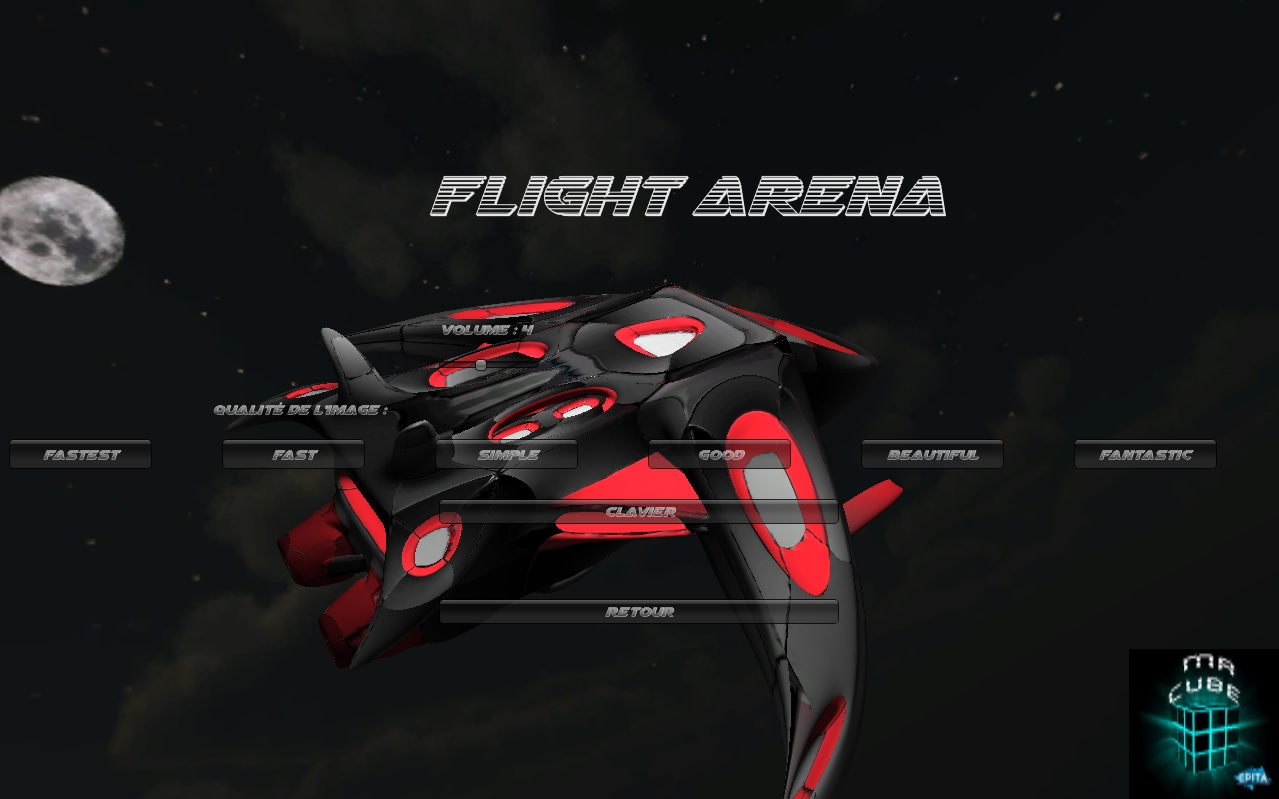
\includegraphics[height=7cm, width=12cm]{menu_option.jpg}
\end{center}

Il a aussi fait en sorte que le joueur puisse choisir le vaisseau qu'il veut piloter parmi les différents proposés avant de commencer la partie parmi les trois proposés faits par Vincent. Ce n'est qu'une différence d'habillage, les trois vaisseaux ont les mêmes propriétés physiques (vitesse, rotation \dots )\\

\begin{center}
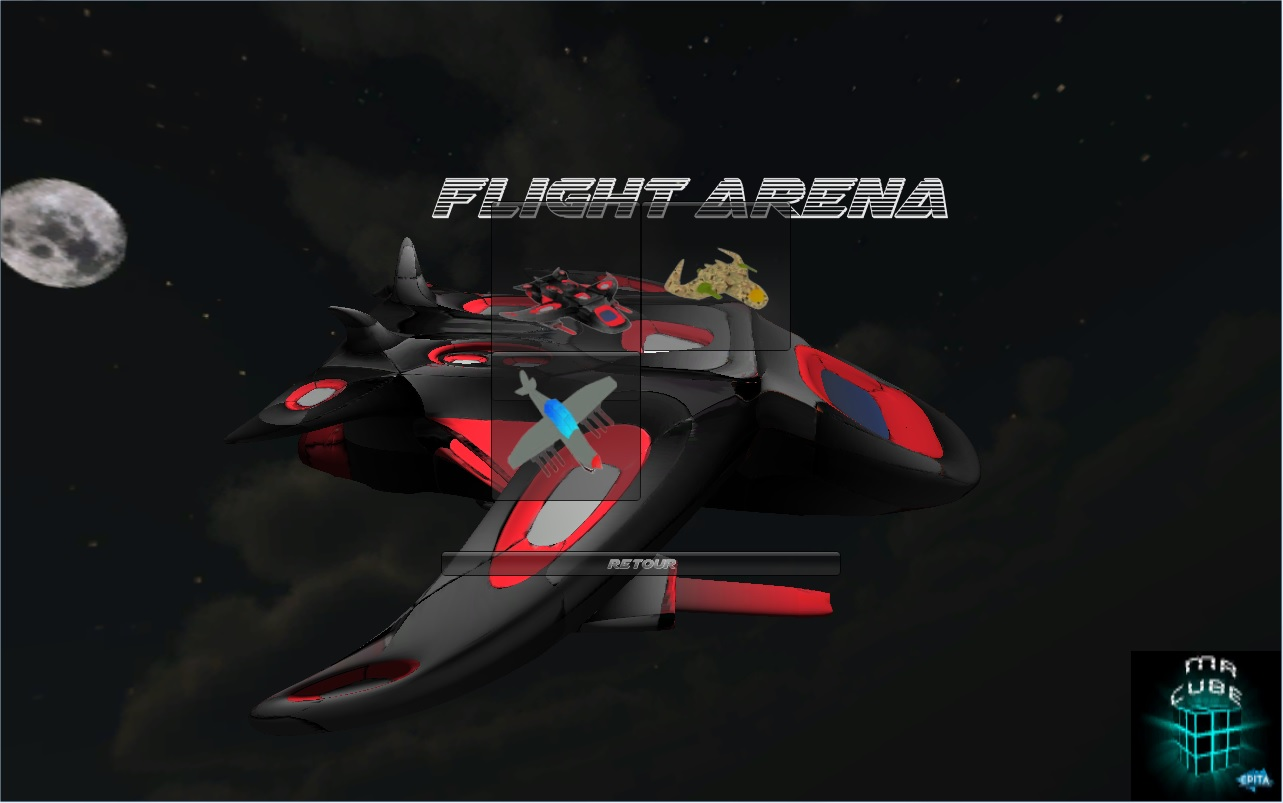
\includegraphics[height=7cm, width=12cm]{menu_selection.jpg}
\end{center}

Au départ, nous voulions faire en sorte que le joueur puisse choisir la répartition des touches de son clavier s'il voulait changer ses commandes pour être plus à l'aise. Cependant, nous ignorons totalement comment le faire et Arthur n'a rien trouvé sur internet pour le faire, même dans la documentation de Unity. Nous avons donc abandonné cette idée, comme nous l'avons dit dans la partie de retard.\\

Il a aussi été rajouté le texte "Chargement..." lors du chargement d'une partie, pour que le joueur comprenne qu'il doit attendre, alors qu'avant il n'y avait aucune indication. Ce n'est qu'un détail mais il a son importance.\\

\subsection{Ce qu'Arthur doit faire pour la soutenance finale}
Pour la dernière soutenance, Arthur va surtout s'occuper de compléter et de terminer l'intelligence artificielle. Elle doit pouvoir rechercher un minimum l'adversaire, voire même esquiver les attaques. Si le temps le permet, il pourra éventuellement faire plusieurs "attitudes" aux vaisseaux gérés par l'ordinateur : plus agressif, plus prudent \dots  etc. Cela les rendrait moins prévisible et plus réaliste, dans le sens plus humain.\\

Si des modifications doivent être apportées au script ou surtout au multijoueur, c'est lui qui s'en chargera, ou au moins qui aidera vu que c'est lui qui s'en ait chargé pour l'instant.\\

En cas de retard, il pourra aider dans l'élaboration des cartes, pour placer les bâtiments et faire un peu de gameplay.

\chapter{Pour la prochaine soutenance}
Pour la dernière soutenance, le projet devra être fini. Nous allons nous concentrer sur l'intelligence artificielle qui est en retard pour qu'elle soit le plus opérationnelle possible.\\

Il y aura aussi du contenu supplémentaire, notamment des cartes, et tout le contenu sera disponible sur le site internet, en ligne.\\

Le jeu sera fournit avec une installation sur CD-ROM, avec une boite prévue à cette effet.\\ \\ \\ \\ \\ \\ \\

\begin{center}
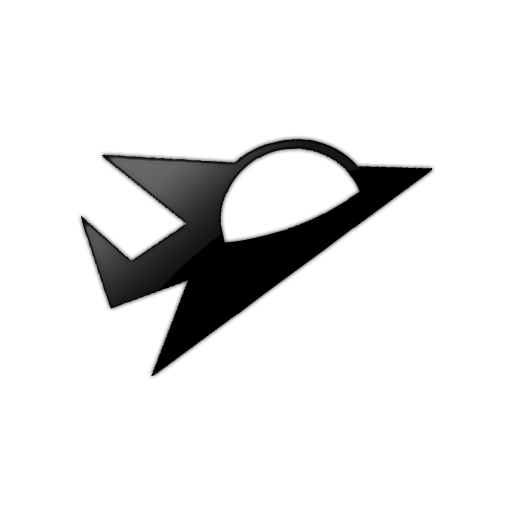
\includegraphics[height=4cm, width=4cm]{vaisseux_petit.png}
\end{center}

\end{document}